\section{Testbox}
\label{sec:testbox}
Der f\"ur Messungen verwendete Testaufbau wurde aus einem vorangegangenen Projekt an der GSI \"ubernommen~\citep{harzheim2016modeling}. Ziel des Testaufbaus war es, eine reproduzierbare Vermessung des Einflusses der MA-Ringkerne auf die Impedanz einer Einkopplung zu erreichen. Dadurch soll eine Absch\"atzung des Einflusses auf die Strahlimpedanz in der Kavit\"at, sowie die Impedanz, welche der \textcolor{red}{Verst\"arker} am Eingang der Kavit\"at sieht, erm\"oglicht werden. Im Rahmen der Bachelorarbeit von Denys Bast am Fachgebiet Beschleunigertechnik~\citep{bast2017ba} wurde f\"ur diese Testbox auch ein Simulationsmodell erstellt. Dieses wird in Abschnitt~\ref{ch:sim} behandelt. 
\par
Die Abmessungen der Testbox sind Abbildung~\ref{fig:boxdimensions} zu entnehmen.
\par
\begin{figure}[htb]
	\centering
	\includegraphics[width=0.6\textwidth]{testbox}
	\caption{Abmessungen der Testbox, alle L\"angenangaben in Millimeter.}
	\label{fig:boxdimensions}
\end{figure}
Mit:\\
H0 = $\SI{600}{\milli\meter}$\\
H1 = $\SI{350}{\milli\meter}$\\
H2 = $\SI{445}{\milli\meter}$\\
H3 = $\SI{595}{\milli\meter}$


\par
Ausgehend von den bestehenden Aufbauten und Modellen wird im Folgenden analysiert, inwiefern ein oder mehrere sekund\"are Kurzschl\"usse die durch den Ringkern verursachte Impedanz reduzieren k\"onnen. 


\newpage


\subsection{Anfangsmessung}
Um eine grobe Tendenz und ein Gef\"uhl f\"ur den Messaufbau zu erreichen wurden zun\"acht einige Messungen an der unmodifizierten Testbox ausgef\"uhrt. Die Testbox selbst besteht aus einem auf Rollen gelagerten Holzrahmen. Dieser ist von innen komplett mit Kupferblech der Dicke $\SI{1}{\milli\meter}$ \"uberzogen. Der Überzug schirmt die Messungen in der Testbox von \"au\ss{}eren Einfl\"ussen ab. Au\ss{}erdem wird damit f\"ur alle Messungen eine identische Umgebung geschaffen, womit diese am Ende vergleichbar bleiben. Um sp\"ater Ringkerne einbringen zu k\"onnen, befindet sich eine Konstruktion aus Holz in der Box, welche als Halterung dient. Diese besteht aus einem Quer- und einem senkrechten Balken, an dem die eigentliche Halterung angeschraubt werden kann. Diese Halterung ist rund und entspricht mit $\SI{260}{\milli\meter}$ dem Innendurchmesser der Ringkerne. Diese k\"onnen dadurch passgenau eingeh\"angt werden. Etwas versetzt zur Mitte der Halterung ist durch ein Loch das Einkopplungsrohr gef\"uhrt, welches mit einem Netzwerk-Analysator verbunden werden kann, um die Feldimpedanz zu messen. Abbildung~\ref{fig:leereBox} zeigt das Innere der Testbox mit eingeh\"angtem Ringkern.
\par
\begin{figure}[htb]
		\centering
		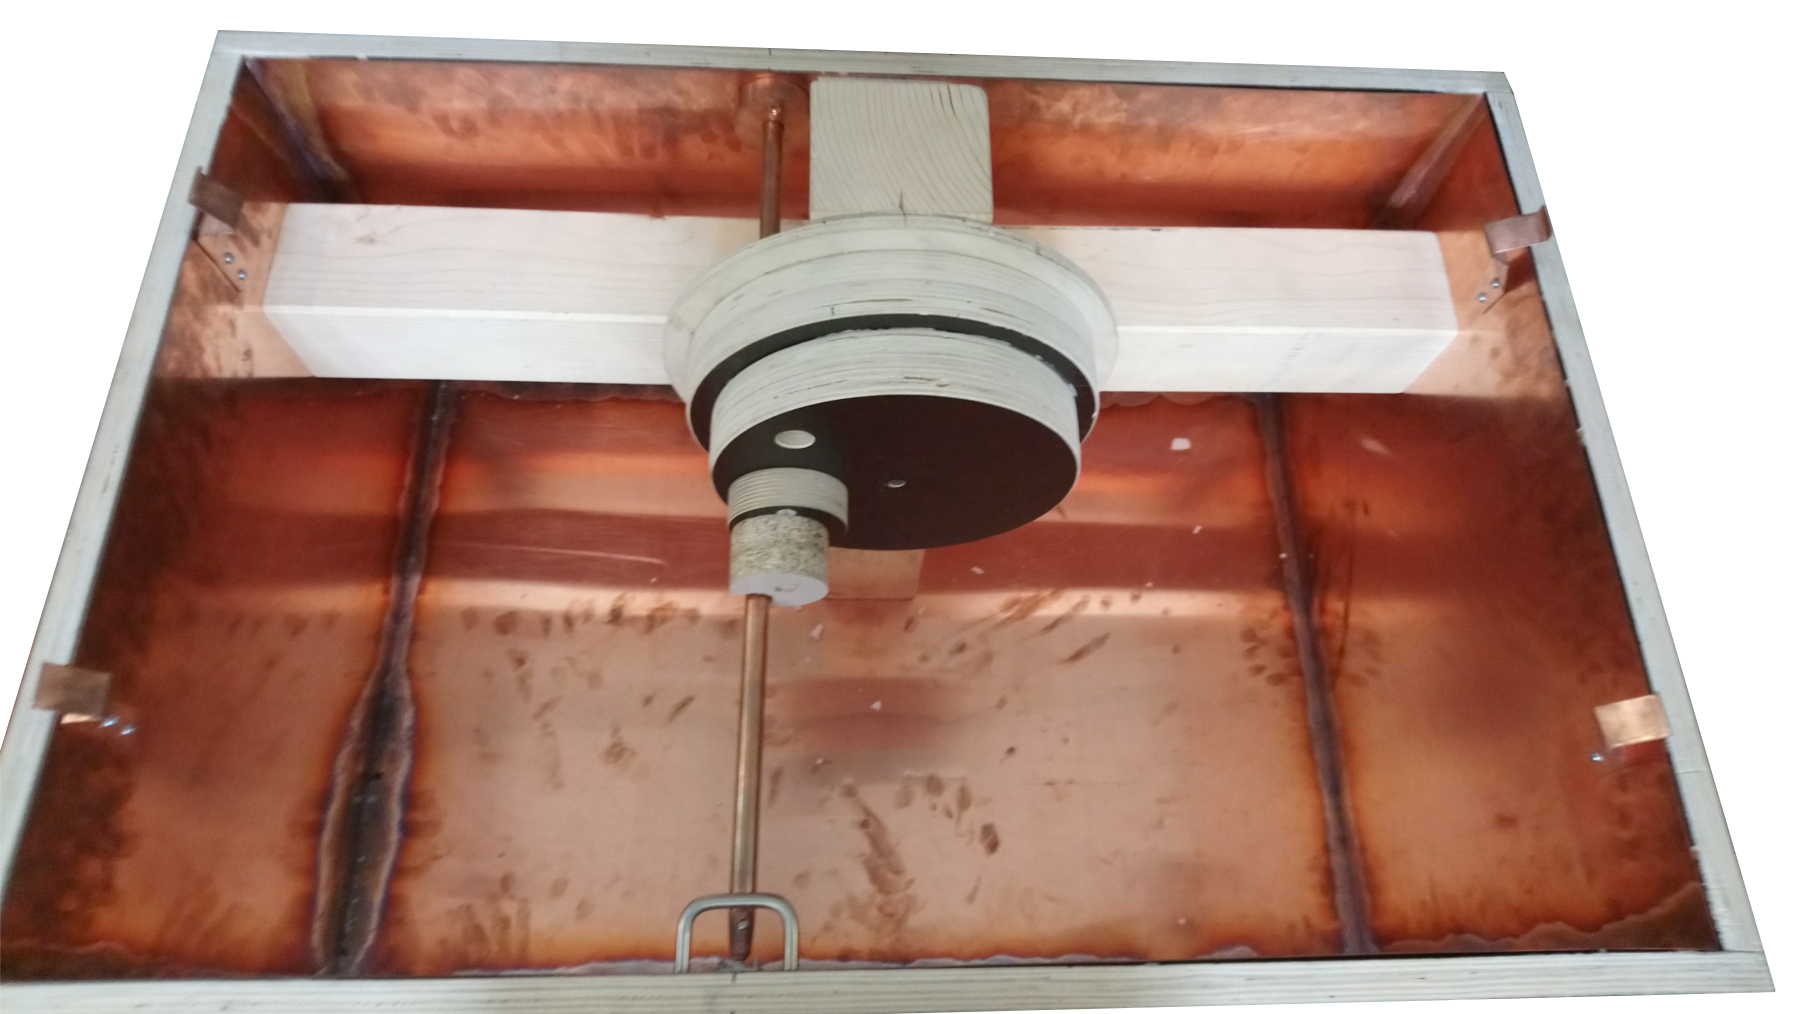
\includegraphics[width=0.5\textwidth]{boxleer}
		\caption{Ge\"offnete Testbox mit Holzkonstruktion als Halterung f\"ur den MA-Ringkern.}
		\label{fig:leereBox}
\end{figure}
F\"ur die ersten Kurzschlussversuche wurden im Test einfache Kupferdr\"ahte mit L\"usterklemmen verwendet. Die Kupferdr\"ahte sind isoliert, sodass diese keinen Kontakt zum Ringkern herstellen. Lediglich die Enden in den Klemmen wurden abgeschliffen, um einen Kontakt herzustellen. Diese Kupferdr\"ahte lassen sich problemlos durch die Bohrungen an der Innenseite des Ringkerns (siehe Abbildung~\ref{fig:innenKern}) f\"uhren, was in Position zumindest an der Innenseite fixiert.
\par
\begin{figure}[htb]
		\centering
		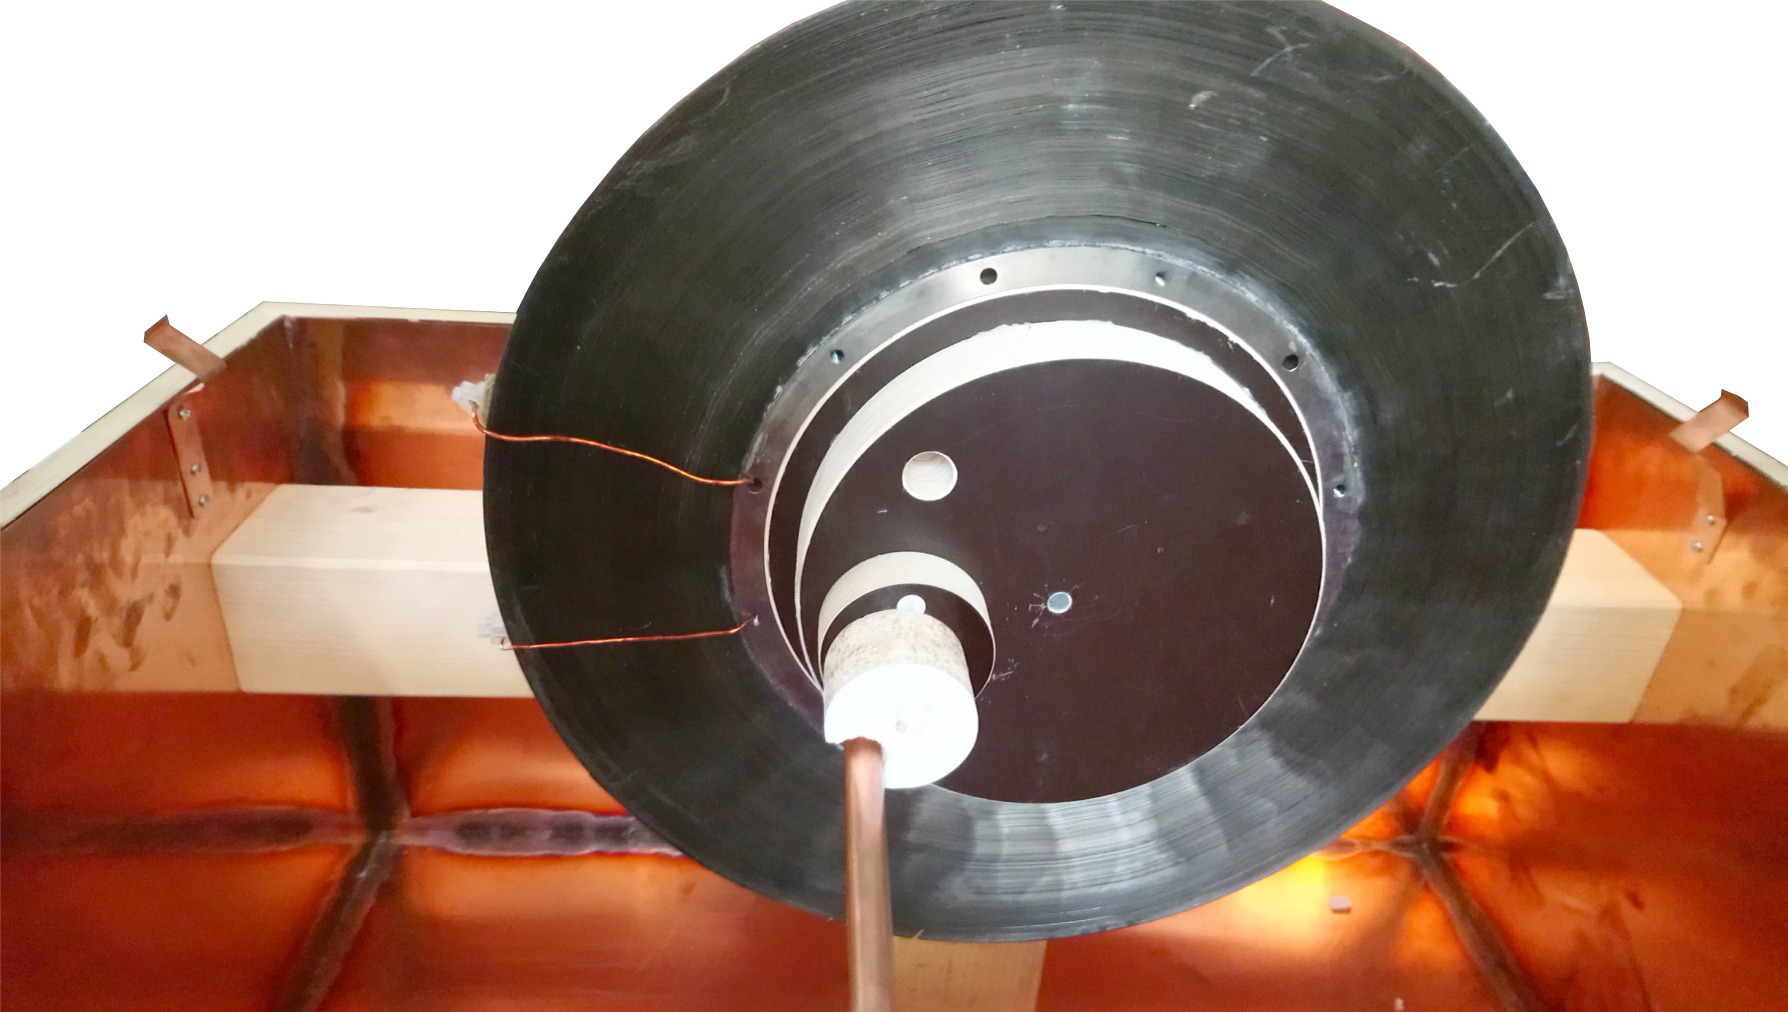
\includegraphics[width=0.6\textwidth]{BoxRKKlemmeKS}
		\caption{Kurzschl\"usse um den Ringekern mittels Dr\"ahten, deren Enden mit L\"usterklemmen verbunden sind.}
		\label{fig:innenKern}
\end{figure}


\newpage


\subsection{Modifikation der Ringkernhalterung}
Um reproduzierbare Messungen durchf\"uhren zu k\"onnen sind mehrere Anforderungen an den Aufbau der Testbox zu stellen. Zun\"achst muss die M\"oglichkeit bestehen, den MA-Ringkern in die Testbox einzubringen, sodass sich dieser bei jeder Messung an der gleichen Position befindet. Des weiteren ist eine M\"oglichkeit zu schaffen, bei der die Kurzschl\"usse an festgelegten  Stellen um den Ringkern zu f\"uhren sind, ohne dass diese den Kern dabei ber\"uhren. Um das zu erreichen wurde die Halterung wie in Abbildungen~\ref{fig:BoxKreuzPolygon} und~\ref{fig:BoxKreuzPolygonRK} modifiziert.


% Zum einen Muss eine Ma\ss{}genaue Halterung f\"ur den Ringkern angebracht werden. Dar\"uber hinaus sollte die Halterung einen Anschlag besitzen, um die Position sicher zu stellen. Abbildung~\ref{fig:BoxKreuzPolygon} zeigt die \"Uberarbeitete Halterung. Das Holzkreuz im hinteren Teil der Halterung ragt einige Millimeter \"uber den Rand des Inneren Halterungsrings hervor. Dieser ist zur Widerstandsf\"ahigkeit Fertigung aus Trovidur~\citep{roechling2016} gefertigt, in diesem Material k\"onnen auch problemlos Gewinde eingeschnitten werden. Der Ring besitzt einen Au\ss{}endurchmesser von $\SI{129}{\milli\meter}$, damit MA-Ringkern mit einem Innenradius von $\SI{130}{\milli\meter}$ leicht und dennoch passgenau montierbar bleibt.

\begin{figure}[htb]
	\centering
	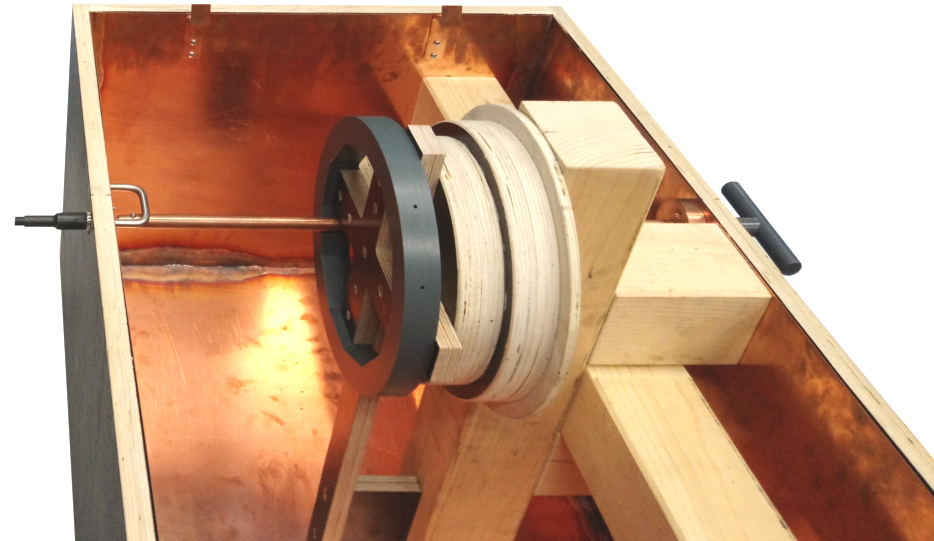
\includegraphics[width=0.65\textwidth]{BoxKreuzPolygon}
	\caption{Halterung aus einem Polygon, welches auf ein Holzkreuz aufgesetzt wurde mit sichtbarem Anschlag.}
	\label{fig:BoxKreuzPolygon}
\end{figure}

Auf der Innenseite des inneren Rings befindet sich ein Polygonzug. Durch diesen Polygonzug k\"onnen Kurzschlussb\"ugel reproduzierbar an festgelegten Positionen platziert werden. Dazu wurden an den Fl\"achenmittelpunkten der inneren Polygonfl\"achen Bohrungen mit einem M4 Gewinde vorgesehen, an dem Kurzschl\"usse montiert werden k\"onnen. Abbildung~\ref{fig:BoxKreuzPolygonRK} zeigt den Polygonzug mit montiertem Ringkern.

\begin{figure}[htb]
	\centering
	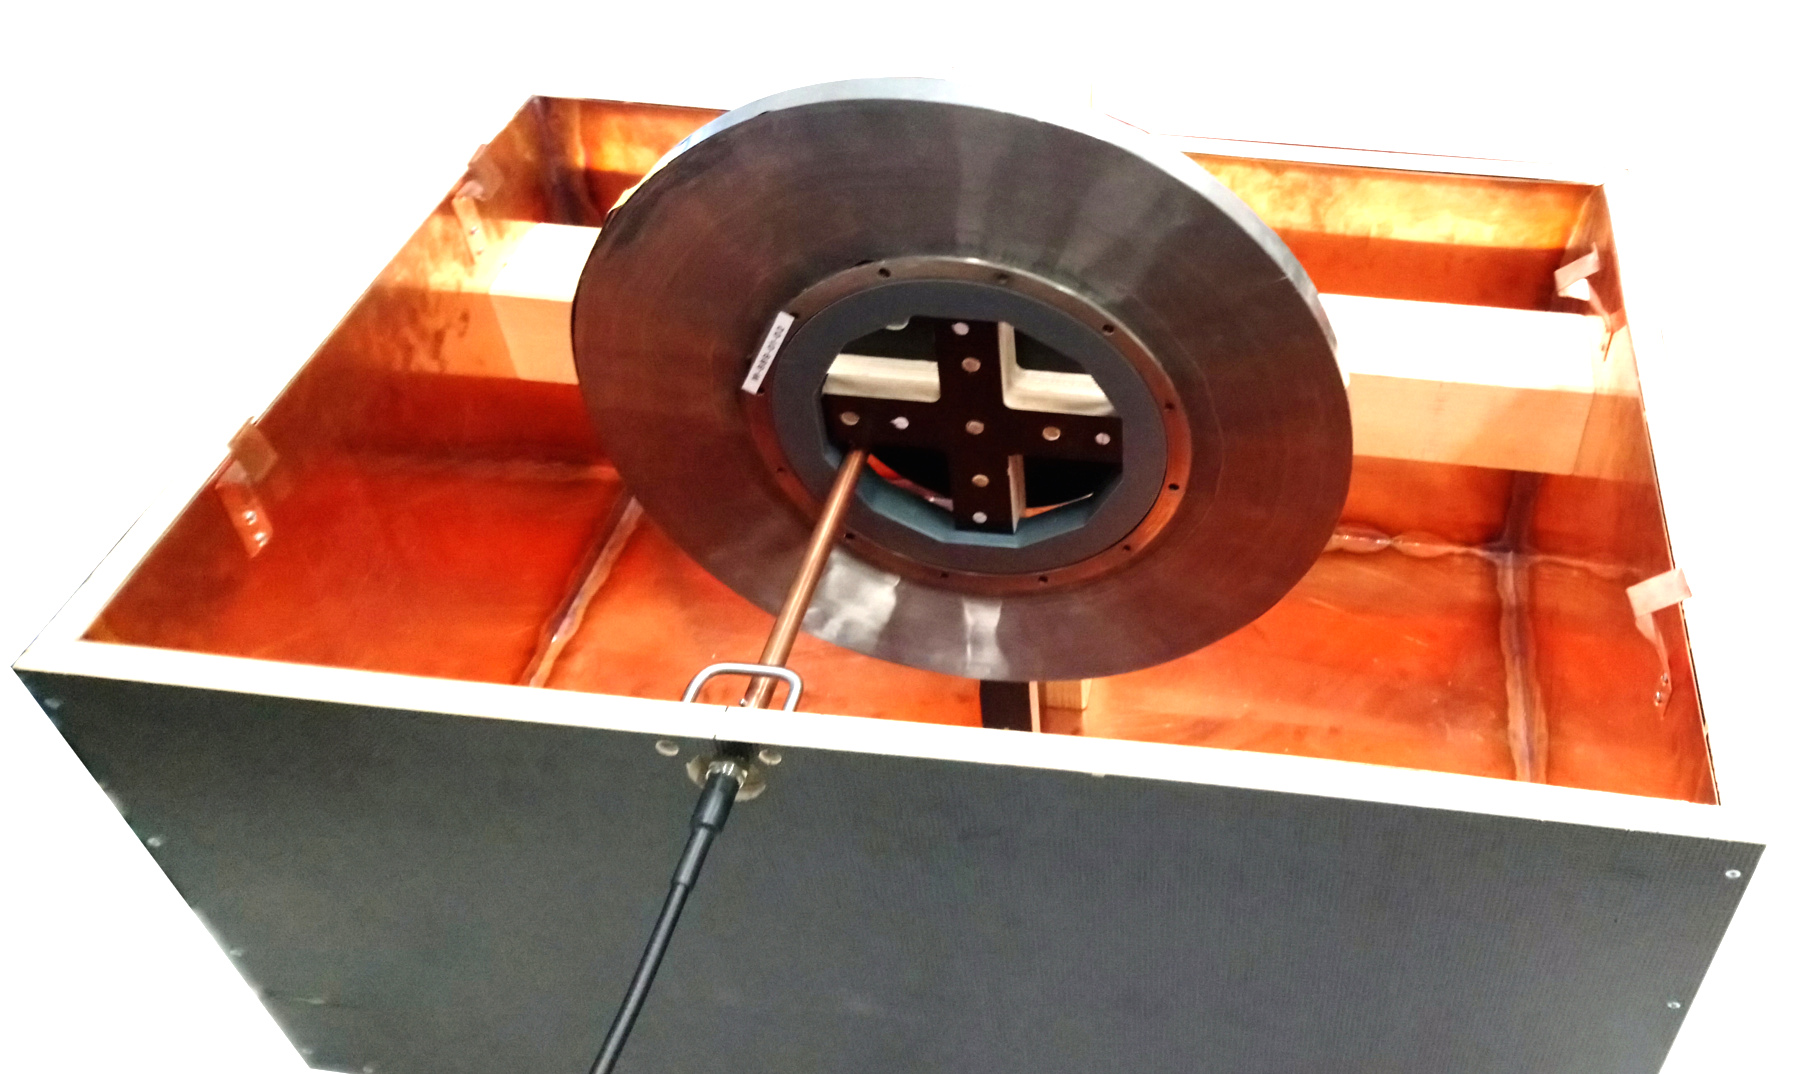
\includegraphics[width=0.75\textwidth]{BoxKreuzPolygonRK}
	\caption{Eingebrachter Ringkern auf der Halterung bestehend aus einem Polygon, welches auf ein Holzkreuz aufgesetzt wird.}
	\label{fig:BoxKreuzPolygonRK}
\end{figure}


\newpage



\subsection{Entwurf der Kurzschlussschienen}
\label{sec:shorts}
Die Kurzschlussschienen selbst sind so zu entwerfen, dass diese unabh\"angig von der Form stets in festgelegter Position an die vorgesehenen Verschraubungen im Polygonzug angebracht werden k\"onnen. Um das zu gew\"ahrleisten, wurden die Schienen genau auf die Geometrie des Polygonzugs angepasst. Abbildung~\ref{fig:TZKS} zeigt eine Beispielhafte Kurzschlussschiene.
\par
\begin{figure}[htb]
	\centering
	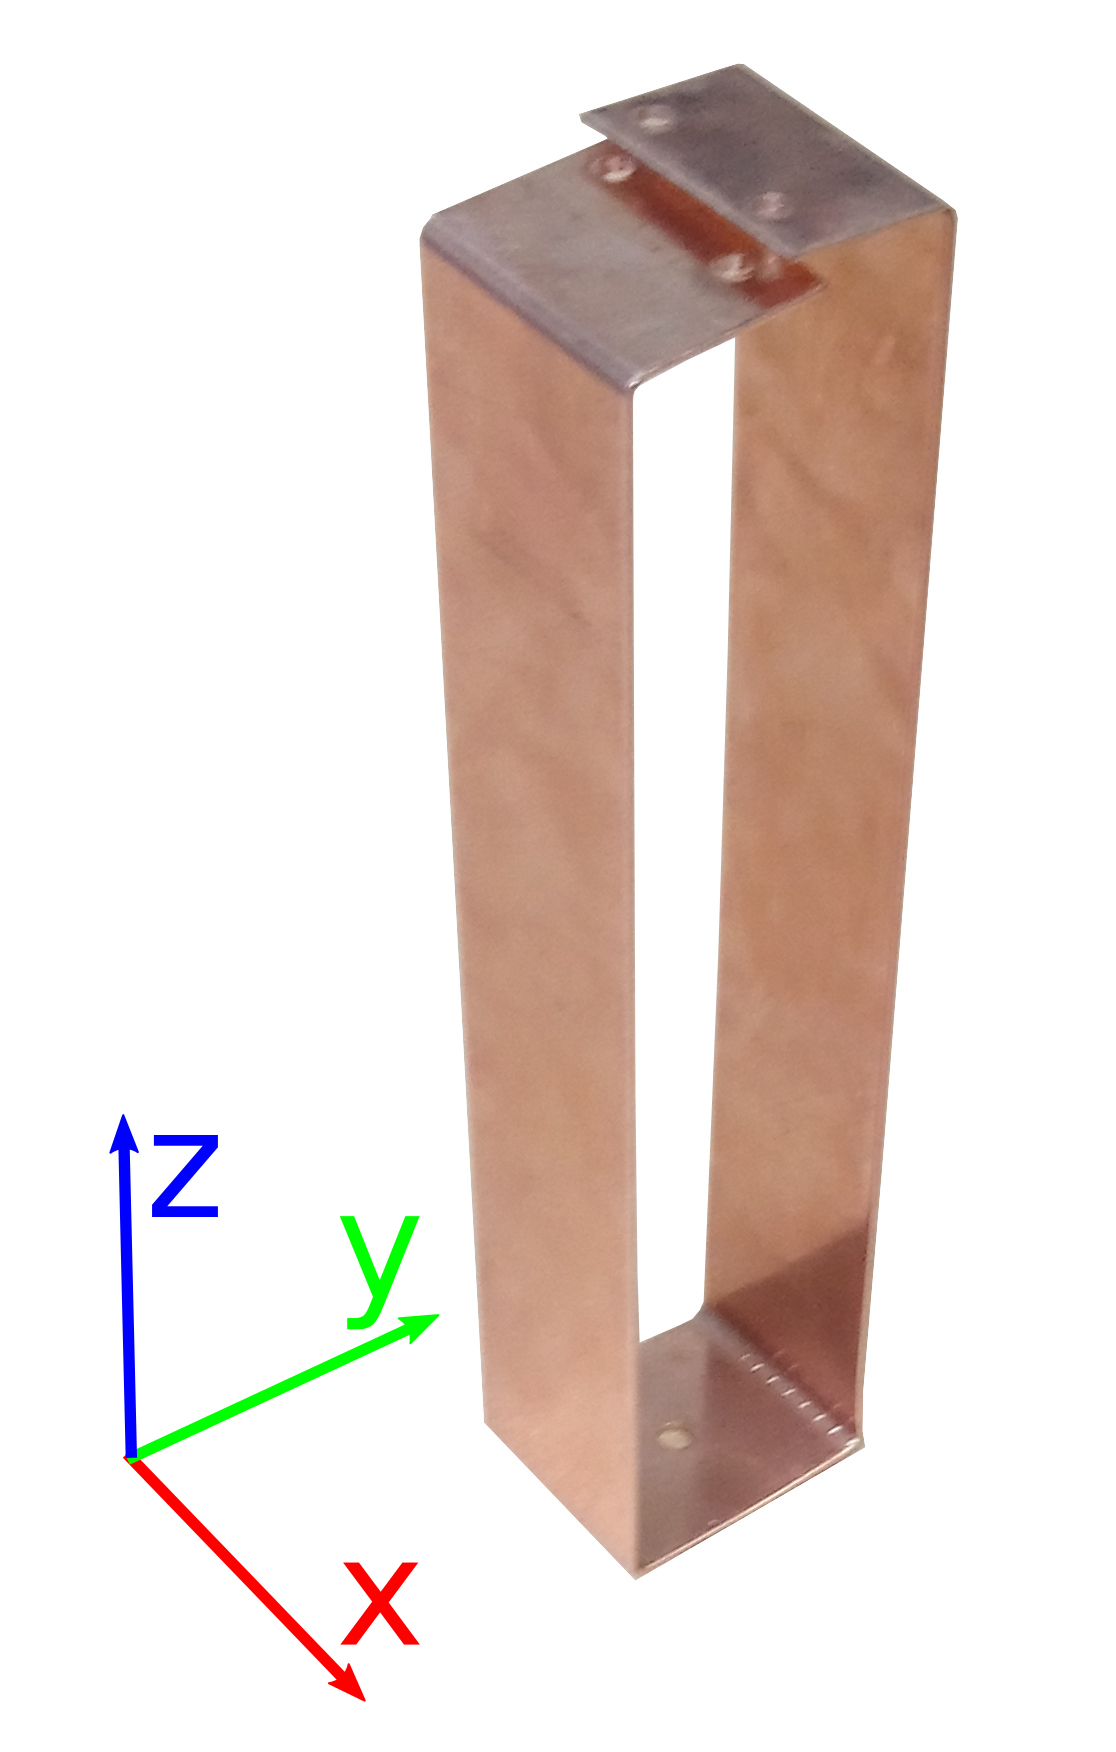
\includegraphics[height=0.4\textwidth]{KS}
	\caption{Kurzschlussschiene mit einer H\"ohe in z-Richtung von $\SI{160}{\milli\meter}$ einer Breite in x-Richtung von $\SI{30}{\milli\meter}$ und einer Blechdicke von $\SI{1}{\milli\meter}$.}
	\label{fig:TZKS}
\end{figure}

Dazu wurden die Kurzschl\"usse jeweils aus einem l\"anglichen St\"uck Kupferblech gefertigt. Diese werden so gebogen, dass die untere Breite (bei z=0) in y-Richtung mit $\SI{30}{\milli\meter}$ genau der Breite des Polygonzugs entspricht. Mittig auf dieser Seite befindet sich ein Loch mit dem Durchmesser $\SI{4}{\milli\meter}$ durch das Blech. Durch dieses kann die Schiene mit dem Polygon verschraubt werden. Zum Schlie\ss{}en der Schienen auf der Au\ss{}enseite befinden sich an beiden Enden des Kupferblechs jeweils zwei L\"ocher, welche nach dem Biegen mit Schrauben und Muttern verbunden werden k\"onnen. Die \"ubrigen Dimensionsgr\"o\ss{}en der Schienen sind folglich variabel die Positionen an der Innenseite sind dabei aber vordefiniert.
\par
Die getesteten Formen der Kurzschl\"usse sind in mehrere Variationsparameter unterteilt:
\begin{itemize}
	\item H\"ohe der Kurzschl\"usse in z-Richtung
	\item Breite der Kurzschl\"usse in x-Richtung
	\item Blechdicke der K\"urzschl\"usse
\end{itemize}



\newpage



F\"ur die Messung wurde eine ganze Reihe an Kurzschlussschienen angefertigt, damit f\"ur jede Form der Schienen unterschiedliche Anzahlen an Kurzschl\"ussen gemessen werden k\"onnen und mehrere Stufen f\"ur jeden Variationsparameter vorhanden sind. Ein Bild aller Kurzschlussschienen ist in Abbildung~\ref{fig:AlleKs} zu sehen.
\par
\begin{figure}[htb]
	\centering
	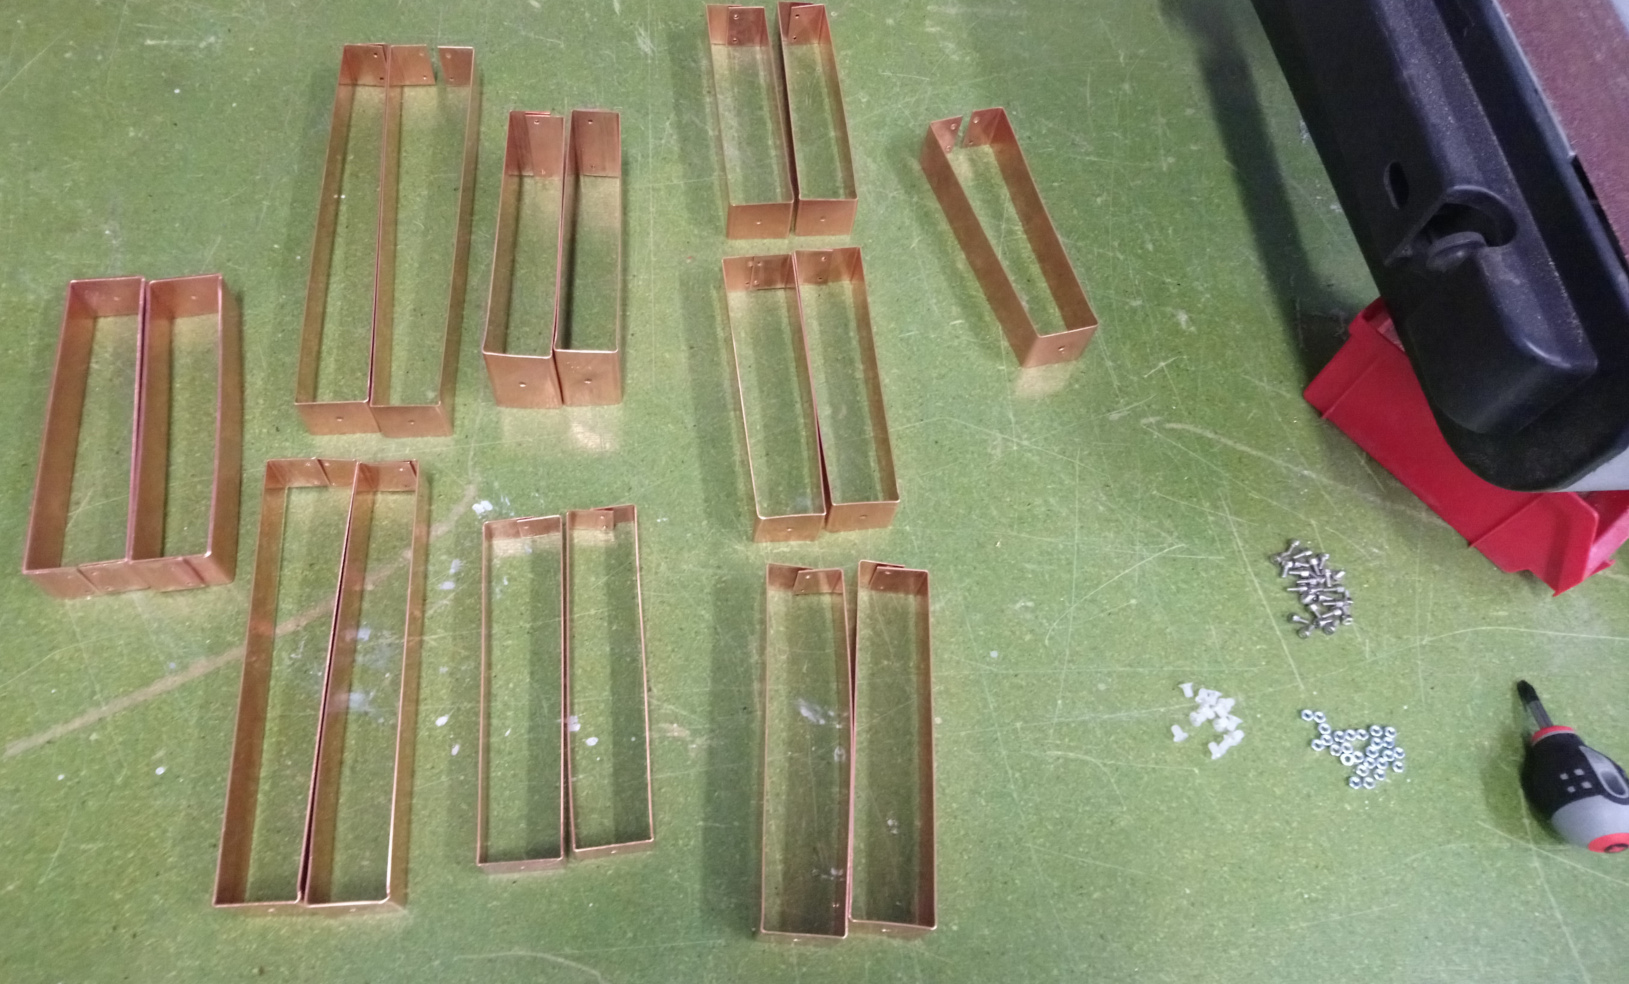
\includegraphics[width=0.65\textwidth]{AlleKs}
	\caption{Alle f\"ur Messungen angefertigte Kurzschlussschienen.}
	\label{fig:AlleKs}
\end{figure}
Insgesamt wurden folgende Kurzschl\"usse angefertigt:
\par
\begin{itemize}
	\item 8x $\SI{160}{\milli\meter}$ H\"ohe in z-Richtung, $\SI{30}{\milli\meter}$ Breite in x-Richtung und $\SI{1}{\milli\meter}$ Blechdicke
	\item 2x $\SI{200}{\milli\meter}$ H\"ohe in z-Richtung, $\SI{30}{\milli\meter}$ Breite in x-Richtung und $\SI{1}{\milli\meter}$ Blechdicke
	\item 2x $\SI{250}{\milli\meter}$ H\"ohe in z-Richtung, $\SI{30}{\milli\meter}$ Breite in x-Richtung und $\SI{1}{\milli\meter}$ Blechdicke
	\item 2x $\SI{160}{\milli\meter}$ H\"ohe in z-Richtung, $\SI{20}{\milli\meter}$ Breite in x-Richtung und $\SI{1}{\milli\meter}$ Blechdicke
	\item 2x $\SI{160}{\milli\meter}$ H\"ohe in z-Richtung, $\SI{50}{\milli\meter}$ Breite in x-Richtung und $\SI{1}{\milli\meter}$ Blechdicke
	\item 2x $\SI{160}{\milli\meter}$ H\"ohe in z-Richtung, $\SI{30}{\milli\meter}$ Breite in x-Richtung und $\SI{2}{\milli\meter}$ Blechdicke
\end{itemize}
Augehend davon wurden insgesamt 18 verschiedene Messungen durchgef\"uhrt, wobei immer nur eine Form der Schienen gleichzeitig montiert wurde.


\newpage



\section{Messdurchf\"uhrung}
Die Messungen werden mit einem Agilent 8753ES~\citep{agilent2000} Netzwerk-Analysator durchgef\"uhrt, der durch ein BNC-Kabels mit der Einkopplung verbunden wird. Um eine unverf\"alschte Messung zu gew\"ahrleisten wird ein verwindungsfestes Kabel genutzt. Somit werden Phasenfehler, welche durch Lage\"anderung des Kabels nach der urspr\"unglichen Kalibrierung entstehen k\"onnen, vermieden. Abbildung~\ref{fig:messstand} bildet diesen Aufbau ab.
\par
\begin{figure}[htb]
	\centering
	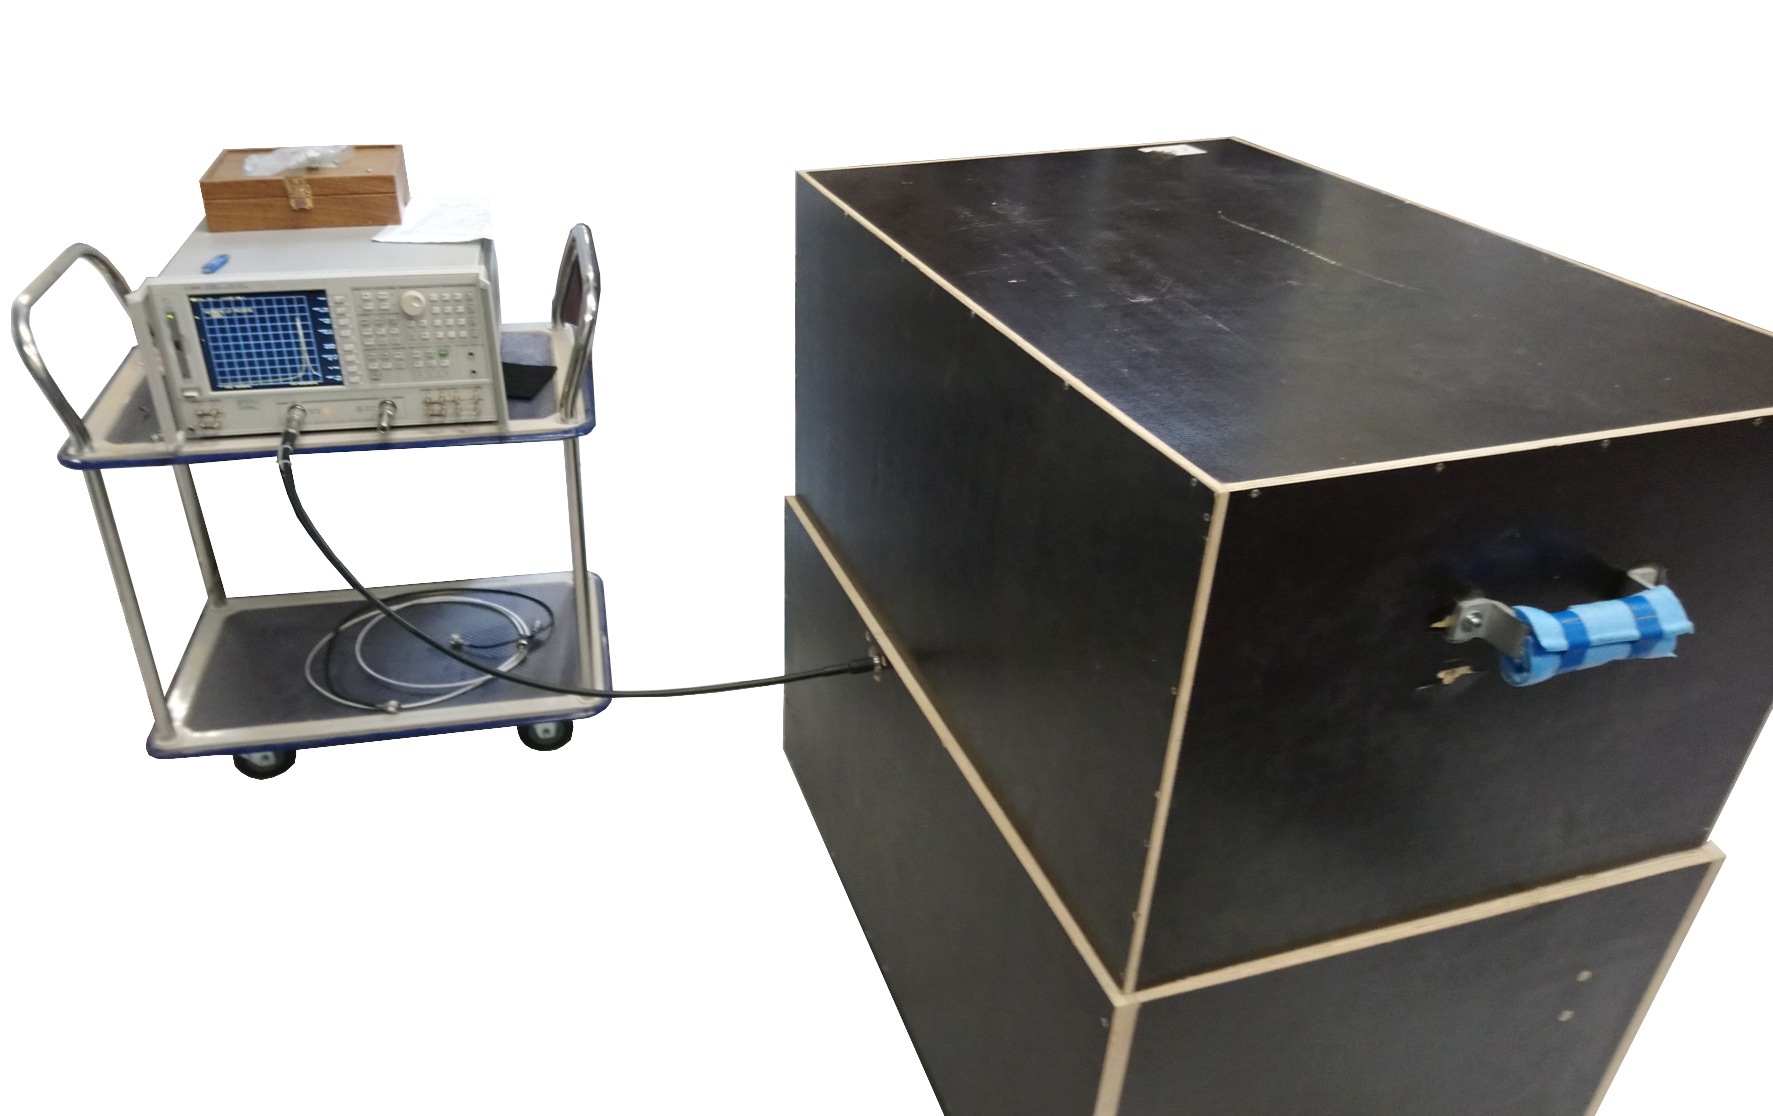
\includegraphics[width=0.75\textwidth]{messstand}
	\caption{Messstand mit Netzwerk-Analysator, welcher mit der geschlossenen Testbox verbunden ist.}
	\label{fig:messstand}
\end{figure}

Dar\"uber hinaus ist zu beachten, dass immer Imagin\"arteil und Realteil der Impedanz getrennt aufgenommen werden, damit bei der sp\"ateren Simulation das RLC-Modell der Testbox \"uberpr\"uft werden kann. F\"ur die Abschlie\ss{}ende Auswertung des Effekts der Kurzschl\"usse wird allerdings nur der Absolutwert der Impedanz f\"ur den Vergleich herangezogen. Der Netzwerk-Analysator nimmt den Frequenzbereich mit einer Aufl\"osung von insgesamt 1601 Messpunkten auf. Der aufgenommene Messbereich erstreckt sich von $\SI{30}{\kilo\hertz}$ bis $\SI{100}{\mega\hertz}$. Daraus ergibt sich eine Messaufl\"osung nach Gleichung~\ref{eq:measureres}.
\begin{equation}
	\frac{\SI{100}{\mega\hertz} - \SI{0,03}{\mega\hertz} }{1601} \approx \SI{62,5}{\kilo\hertz} 
	\label{eq:measureres}
\end{equation}


